 \documentclass[12pt]{article}
 
\usepackage[margin=1in]{geometry} 
\usepackage{amsmath,amsthm,amssymb}
\usepackage{graphicx}
\usepackage{hyperref}
\usepackage{fancyhdr}

\pagestyle{fancy}

%\lhead{\href{https://github.com/hanuka24/ActMonitoringLocalizationApp}{Link} to our repository}

\begin{document}
 
\title{Mobile Computing, Lab}
\author{Hannah Brunner, Markus Gallacher}

\maketitle


We have made one single App to perform activity monitoring and localization. 

\section{Introduction}

The aim of the course was to implement an Android app which utilizes and processes on-phone sensor data. 

The source code is available on Github \cite{repo}.

\section{Implementation}
\subsection{Main App}
We split the work in such a way that we could work mostly in separate classes to not interfere with each other too much when merging. However most of the time we still worked side by side and we always new what the other one was programming as we revised each others code together.

\begin{center}
  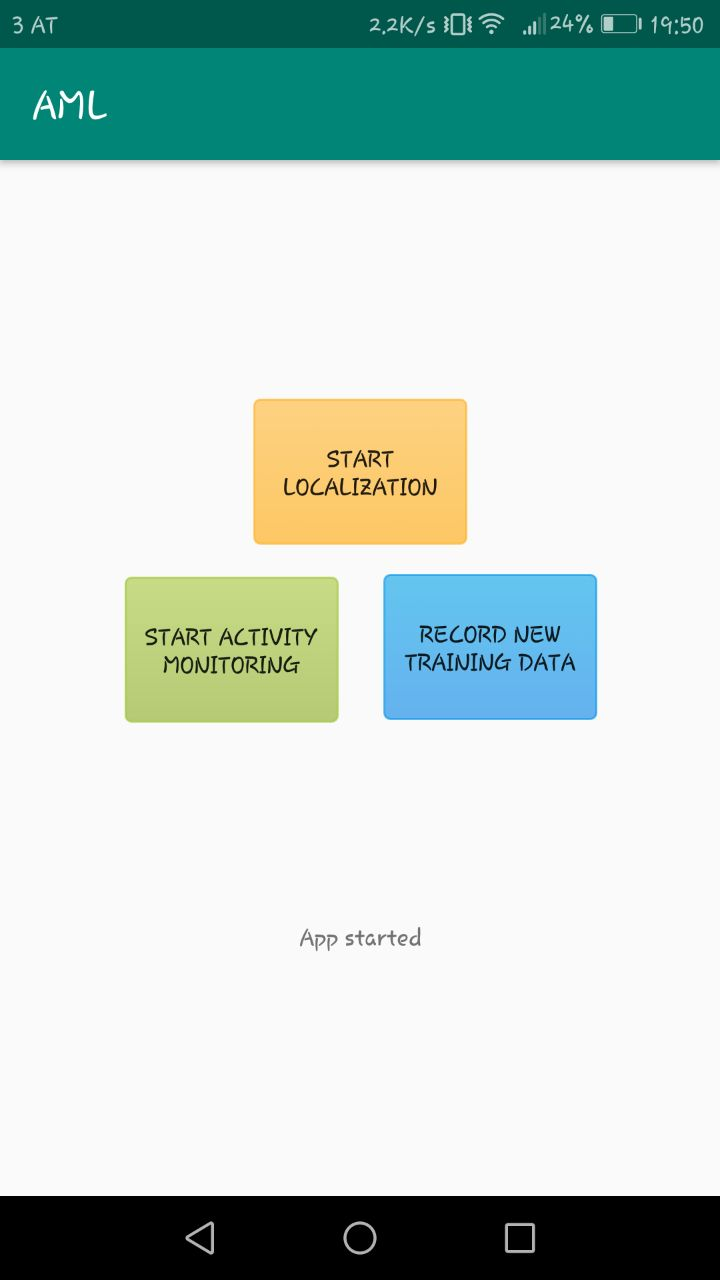
\includegraphics[width=140px]{images/main.jpeg}
\end{center}

\pagebreak

\subsection{Activity Monitoring}
The Activity Monitoring is split into two activities, one collects training data and stores it into a file locally. The other activity monitors the sensors and uses the kNN algorithm to classify the user's motion.

\subsubsection{Background: Activity monitoring using KNN}
kNN is a very simple algorithm which finds the k nearest neighbour in a data set by calculation the euclidean distance between two points. The algorithm is fast and reasonably accurate if enough training data is available and if the k is set appropriately. Wen take the mean of each axis and calc

\subsubsection{Train Activity}
This activity enables the user to collect training data for the monitoring activity. 1 of 4 activities are currently implemented, however any activity can be trained, only the label would mismatch at the moment.
\\
The user needs to press one of the activities and perform the motion. The accelerometer data is sampled over a predefined window and the timestamp, mean of the x, y and z axis as well as the minimum and maximum of the euclidean distance is stores in a local .txt file. The most dominant frequency is also stored but it is currently not used as it lowers the recognition accuracy.
\\
If a faulty measurement was recorded the user can delete the last entry or delete the whole .txt file.

\begin{center}
  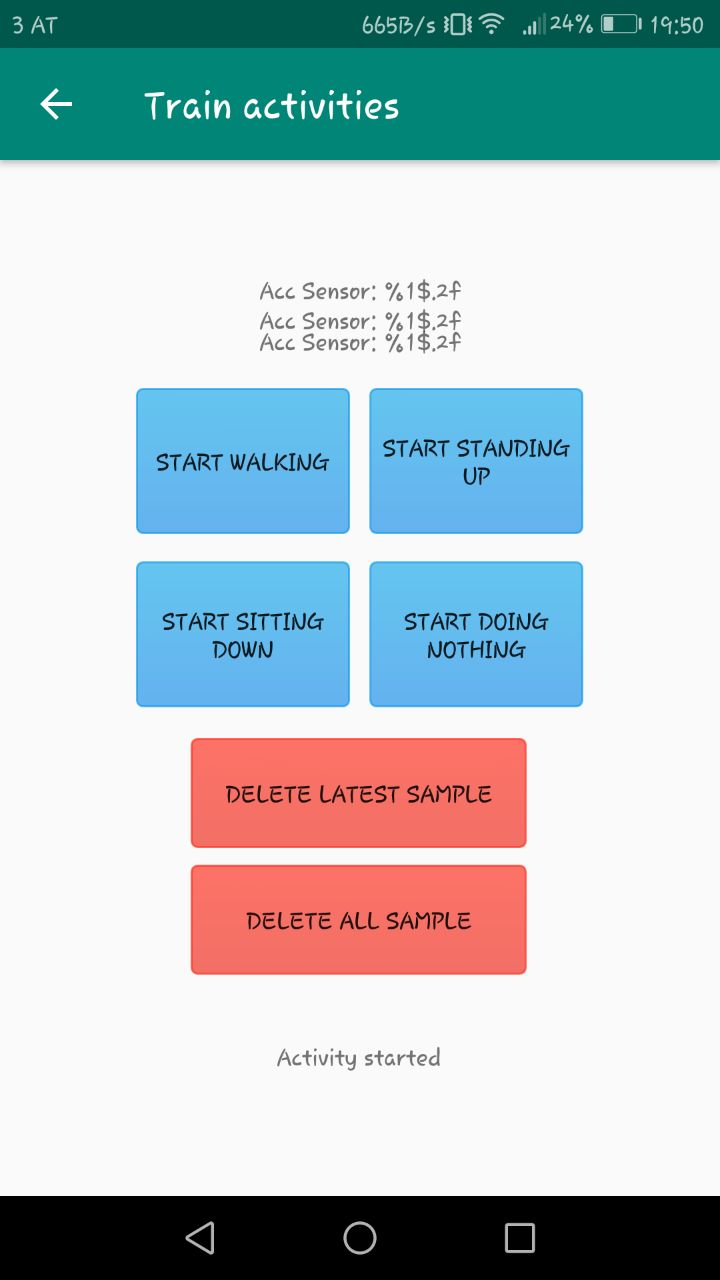
\includegraphics[width=140px]{images/train_activity}
\end{center}

\pagebreak

\subsubsection{Monitoring}


The second activity tries to classify the activity currently performed by the user. When the button is pressed, the accelerometer data is sampled with the same window size as the training data. 
\\
Then a kNN algorithm finds the nearest neighbours by calculating the euclidean distance of the averaged coordinates to each training record and selecting the k closest ones. 
\\
Then we classify the neighbours by weighting each label and adding the weights if a label occurs more than once. This gives us a probability of how certain we are of our match. The recognized activity is displayed together with the probabilities for each of our 4 predefined activities.
\\
When the "continuous monitoring" box is ticked, this prediction process (sample, kNN, classify) is repeated endlessly.

\begin{center}
  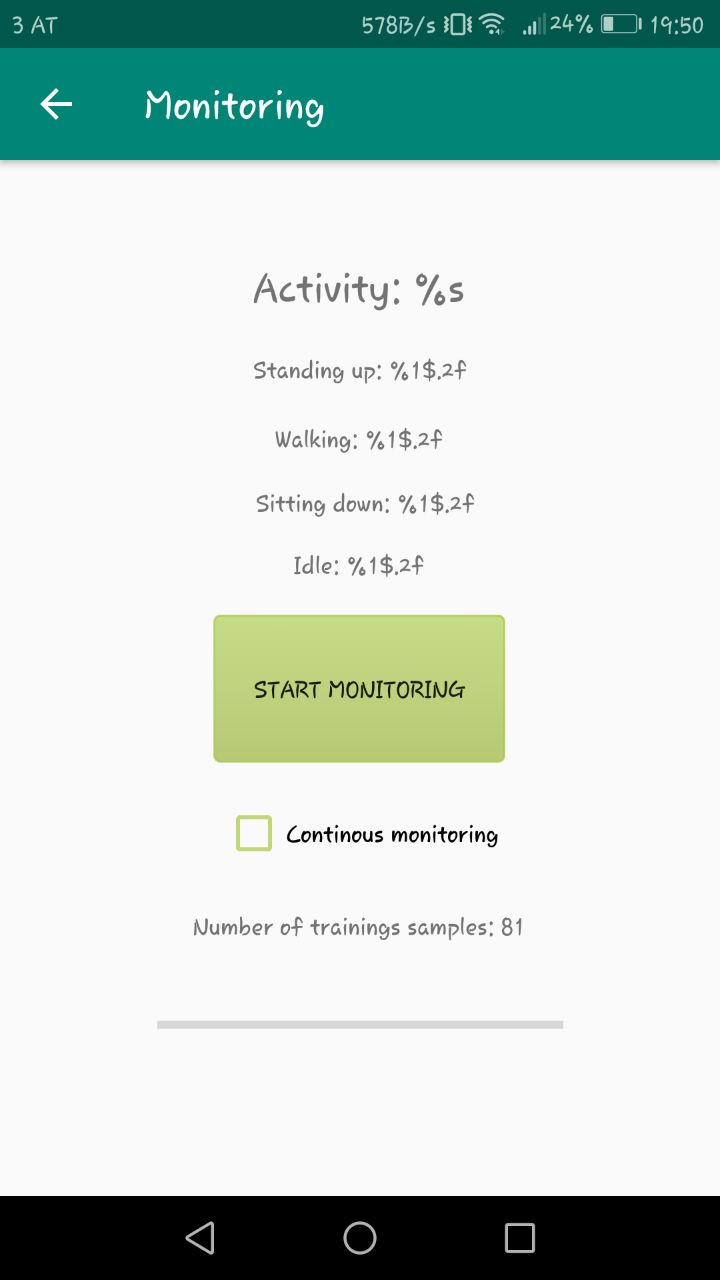
\includegraphics[width=140px]{images/monitoring.jpeg}
\end{center}

\pagebreak

\subsubsection{Limitation/Challenges}

%Python script, accuracy etc.

\subsection{Localization}

\begin{center}
	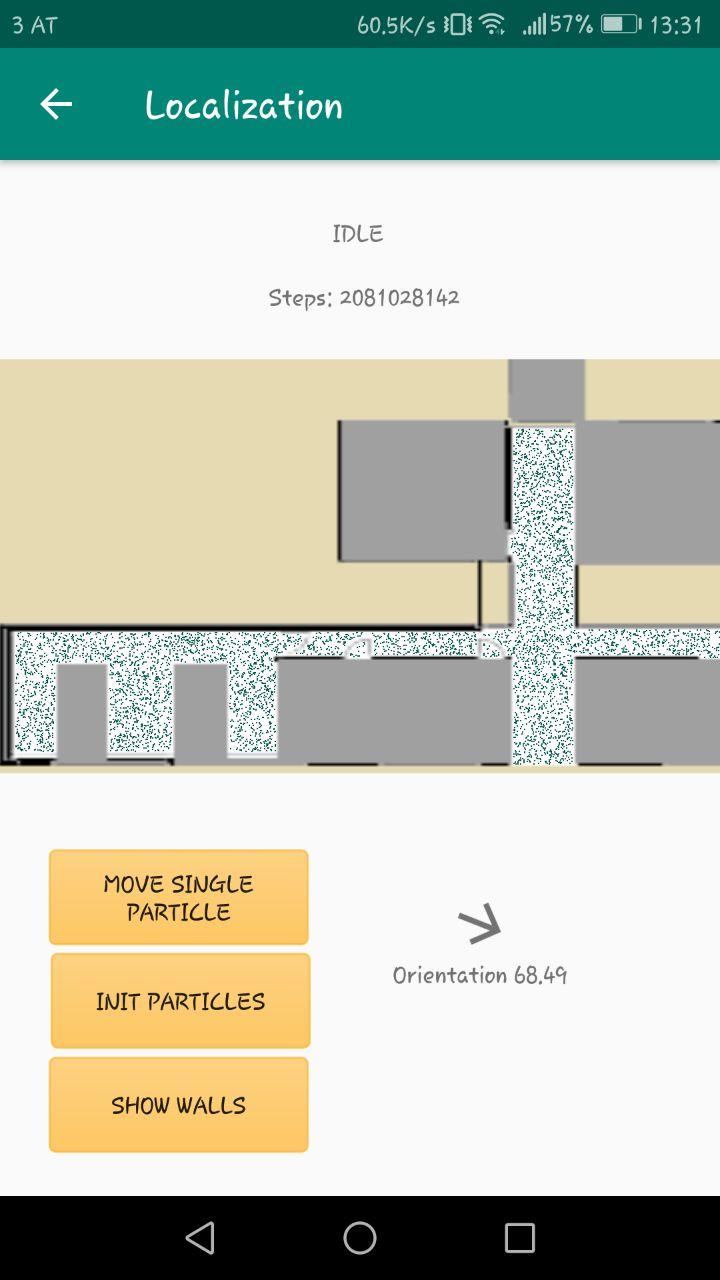
\includegraphics[width=140px]{images/localization}
\end{center}

\subsubsection{Background: Particle Filter}

\subsubsection{Implementation}

\subsubsection{Limitations/Challenges}
%Compass
\bibliographystyle{ieeetr}
\bibliography{refs}


\end{document}